This section introduces the covering problem that does not have any axis-parallel constraint for the ellipses, we denote this version of the problem as \sigla{MCER}{Maximal Covering by Ellipses with Rotation}. The removal of this constraint introduces a new variable which is responsible for determining the rotation angle of every ellipse.

An instance of the non-axis-parallel is defined exactly like the axis-parallel one on \autoref{chapter:ellipses}. It is given by a set of demand points $\Pp=\{p_1, \dots, p_n\}$, with every point having a unitary weight, and a set of ellipses $\E=\{E_1, \dots, E_m\}$, with fixed shape parameters $(a_i, b_i) \in \R^2_{>0}$, $i \in \{1, \dots, n\}$ with the additional condition that $a_i > b_i$. Given an instance of $MCER$, we define $Q:=(q_1, \dots, q_m) \in \R^{2m}$ to be the centers of each ellipse, $\Theta:=(\theta_1, \dots, \theta_m) \in [0, \pi)^m$ to be the angle of rotation of each ellipse and $E_i(q_i, \theta_i)$ to be the coverage region of ellipse $E_i$ with its center at point $q_i$ rotated by angle $\theta_i$, which is given by \autoref{eq:rotated_ellipse_co}.
Also, $\Pp \cap E_i(q_i, \theta_i)$ is denoted as the set of points covered by $E_i$ on this configuration. Therefore MCER is defined as the problem of determining $Q$ and $\Theta$ (placing and rotating each ellipse) to maximize the number of points covered by the $m$ ellipses, which is given by \autoref{eq:optMCEn}.

\begin{equation}\label{eq:optMCEn}
\max_{Q, \Theta}{\left|\bigcup_{i=1}^{m} \Pp \cap E_i(q_i, \theta_i)\right|}.
\end{equation}

An additional notation is used on this chapter, $\tilde{E_i}(q_i, \theta_i)$ is defined to be the set of points on the border of $E_i(q_i, \theta_i)$, specially, the operation $\Pp \cap \tilde{E_i}(q_i, \theta_i)$ is used to refer to the set of points from $\Pp$ that lie on the border of $E_i(q_i, \theta_i)$.


\begin{proposicao}\label{lema:mce_2b}
	Let $(\Pp, \E)$ be an instance of MCER. In an optimal solution of MCER, for any $E_j \in \E$, such that $|\Pp \cap E_j(q_j, \theta_j)|\ge2$, there is $q_j'$ such that $\Pp \cap E_j(q_j', \theta_j)=\Pp \cap E_j(q_j, \theta_j)$ and $\Pp \cap \tilde{E_j}(q_j', \theta_j) \ge 2$.
\end{proposicao}

\begin{demonstracao}
	First, the angle of rotation can be ignored as it does not change.
	
	Let $A=\Pp \cap E_j(q_j, \theta_j)$ be the set of points covered by $E_j$ and $X=\cap_{p \in A}E_j(p, \theta_j)$ be the region of intersection of ellipses centered at each point from $A$.

	As it was shown on \autoref{chapter:ellipses}, $X$ is a region that is limited by arcs of ellipses. As this region is the non-empty intersection of more than one ellipse, there are at least two of these arcs that encounter at one point creating a vertex. Selecting any of these vertices as $q_j'$ will make $|\Pp \cap \tilde{E}_j(q_j', \theta_j)| \ge 2$.
	
\end{demonstracao}

What \autoref{lema:mce_2b} is saying is that any optimal solution for MCER can be transformed into another optimal solution where every ellipse covers the same set of points and those which cover more than one point has two points on their border. Also, this equivalent optimal solution can be always achieved by just translating the ellipses. An example is shown on \autoref{fig:ellipse-2-points} for one ellipse.

A lot of the ideas developed in this chapter are based on fixing two points on the border of an ellipse, which is why \autoref{def:feasible_angle} introduces a new notation for angles that an ellipse rotated by it can be translated into a center, such that it contains two fixed points. 

\begin{figure}[H]
	\centering
	\caption{An optimal solution before and after applying \autoref{lema:mce_2b}.}
	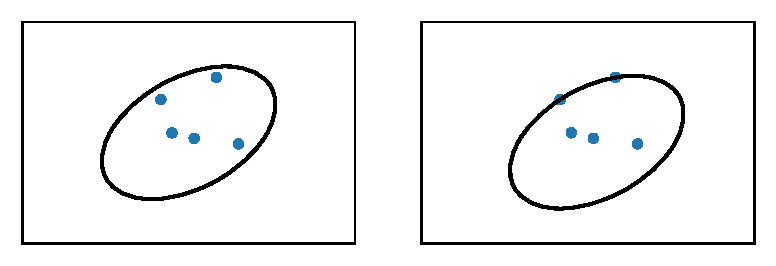
\includegraphics{tex/figures/scripts/ellipse-2-points}
	\fautor
	\label{fig:ellipse-2-points}
\end{figure}



\begin{definicao}\label{def:feasible_angle}
	Let $E$ be an ellipse and $u, v \in \R^2$. An angle $\theta \in [0, \pi)$ is said to be $(E, u, v)$-feasible if there is $q \in \R^2$ such that $\{u, v\} \subset \tilde{E}(q, \theta)$.
\end{definicao}

On \autoref{fig:feasible-angle} two examples for \autoref{def:feasible_angle} are shown. On one of them, an ellipse is rotated by $\pi/4$ and it is located such that it contains the two fixed points on its border. That means $\pi/4$ is a $(E, u, v)$-feasible angle. On the other example, the ellipse is rotated by $\pi/2$ and there is not a center where the ellipse can be placed so it contains the two fixed points--they are too far apart. This makes $\pi/2$ a not $(E, u, v)$-feasible angle.

\begin{figure}
	\centering
	\caption{A $(E, u, v)$-feasible angle and a not $(E, u, v)$-feasible angle.}
	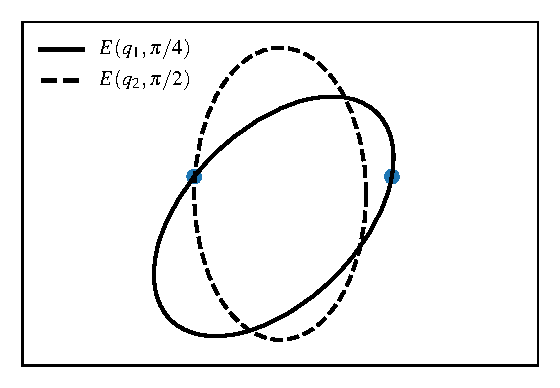
\includegraphics{tex/figures/scripts/feasible-angle}
	\fautor
	\label{fig:feasible-angle}
\end{figure}

\begin{lema}\label{lema:3pnts}
	Let $(\Pp, \E)$ be an instance of MCER, in an optimal solution, for any $E_j \in \E$, such that $|\Pp \cap E_j(q_j, \theta_j)|>2$, at least one of the two cases is true:
	
	\begin{enumerate}
		\item There is $q', \theta'$, and $\{u, v, w\} \subset \Pp \cap E_j(q_j, \theta_j)$, such that $\{u, v, w\} \subset \tilde{E}(q', \theta')$.
		
		\item Let $A=\Pp \cap E_j(q_j, \theta_j)$, and $u, v \in A$ such that there exists $\hat{q}_j$ such that $\{u, v\} \subset \tilde{E_j}(\hat{q}_j, \theta_j)$ and $A \subset E_j(\hat{q}_j, \theta_j)$. Then for any $(E_j, u, v)$-feasible angle $\theta \in [0, 2\pi]$, there exists $\bar{q}_j$ such that $\{u, v\} \subset \tilde{E_j}(\bar{q}_j, \theta)$ and $A \subset E_j(\bar{q}_j, \theta)$.
	\end{enumerate}
\end{lema}

The first case of \autoref{lema:3pnts} is saying that there is another optimal solution which has $E_j$ covering the same set of points, but with three points on its border. 

The second case of \autoref{lema:3pnts} says that after fixing a pair of points on the border of $E_j$ maintaining the covered set, for any angle that allows the two points to stay on the border of $E_j$, there is a center that maintains the covered set the same.

On \autoref{fig:lema-3-points} both cases of \autoref{lema:3pnts} are shown. There, it can be seen that for the second case, it does not matter which feasible angle by which the ellipse is rotated, the third point will always be inside the coverage area. Also, an example of the first case is shown where there are three points lie exactly on the border of the ellipse.

\begin{figure}
	\centering
	\caption{An example of \autoref{lema:3pnts}.}
	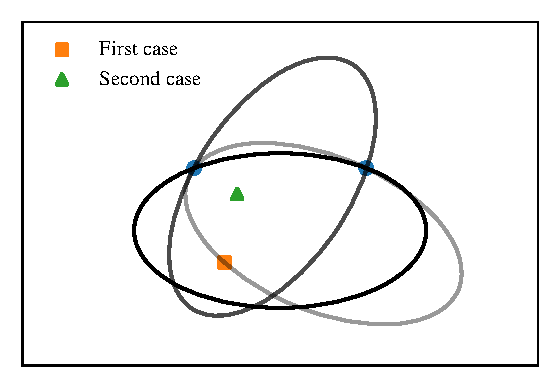
\includegraphics{tex/figures/scripts/lema-3-points}
	\fautor
	\label{fig:lema-3-points}
\end{figure}

The idea to prove \autoref{lema:3pnts} is that after fixing $u, v$ on the border of $E_j$, which is possible by \autoref{lema:mce_2b}, the movement of rotation and translation while keeping $u, v$ on the border is continuous. Because of that, the negation of case two implies case one and vice versa.


If we define an equivalence relation between optimal solutions as: $S_1$ is equivalent to $S_2$ if they both cover the same set of points, we can use \autoref{lema:3pnts} and \autoref{lema:mce_2b} to identify the equivalence classes. Let $S$ be any optimal solution, in $[S]$ (its equivalence class) there is another solution where any ellipse $E_j \in \E$ falls in at least one of the cases below:
\begin{itemize}
	\item $E_j$ covers only one point.
	\item $E_j$ covers more than one point with $u$ and $v$ being on the border of $E_j$. Note that there could be infinitely many of solutions like that, however, \autoref{lema:3pnts} guarantees that any $(E_j, u, v)$-feasible angle yields an equivalent optimal solution.
	\item $E_j$ covers more than two points with three of them on its border.
\end{itemize}

The following two sections will treat the second and third cases (the first case is trivial). Going through every possibility of an ellipse falling in any of the three cases guarantees that an optimal solution is found.

\section{Ellipse by two points}

Let $E$ be an ellipse with shape parameters $(a, b)\in \R^2_{>0}$ and $u, v\in \R^2$, one wants to find a $(E, u, v)$-feasible angle $\theta\in[0,\pi]$ and every center $q\in\R^2$ such that $\{u, v\} \subset \tilde{E}(q, \theta)$.

For a fixed angle, finding every center such that two points are on the border of the ellipse is done on \autoref{chapter:ellipses_intersection}, from there we know that there could be at most $2$ of such centers. The only thing left to be done is finding a feasible angle. It turns out that the angle that makes the major-axis of the ellipse to be aligned with the line that passes through $u$ and $v$ will be a feasible angle if, and only if the set of feasible angles is not empty. This can be seen geometrically as other angles achieve a lesser maximum distance between the two points on the border.

\section{Ellipse by three points}

The problem of finding every center and angle of rotation of an ellipse which makes it have three points on its border is presented in this section. We refer to it as \sigla{E3PNT}{Ellipse by Three points}, and an instance of it is given by three points $u, v, w \in \R^2$ and $E$, an ellipse with shape parameters $(a, b) \in \R^2_{>0}$, with $a > b$. The objective is to find every pair $(q, \theta) \in \R^2\times[0, \pi]$, such that $\{u, v, w\} \subset \tilde{E}(q, \theta)$.

Firstly, it is going to be shown that the number of solutions of E3PNT is limited by a constant, this is a fundamental result which allows an algorithm for MCER to be developed. Secondly, a method to find every solution of E3PNT is described.

\subsection{The number of solutions is limited by a constant}

To prove that the number of solutions is limited by a constant, the problem is going to be modeled as finding the roots of an univariate polynomial of degree $12$.

To make it simpler, let us translate the system, so the point $u$ is at $(0,0)$. Then, we assume that the ellipse is actually axis-parallel and the points are the ones rotating. When an angle is found such that the three points lie on the border of the axis-parallel ellipse, a linear transformation can be applied to compress the x-axis by $\frac{b}{a}$, transforming the ellipse into a circle of radius $b$. This transformation can be seen on \autoref{fig:circumscribed-circle} where a solution of the E3PNT is transformed into a solution of the problem of finding a circumscribed circle of a triangle. 
This process can be parametrized by the angle of rotation of the points, as described by \autoref{eq:trpnts}, and because of the invertibility of linear transformations solutions for E3PNT can be obtained by reversing the transformations.

\begin{figure}[H]
	\centering
	\caption{Transforming an ellipse into a circle. T1, T2, and T3 represent the steps of the transformation.}
	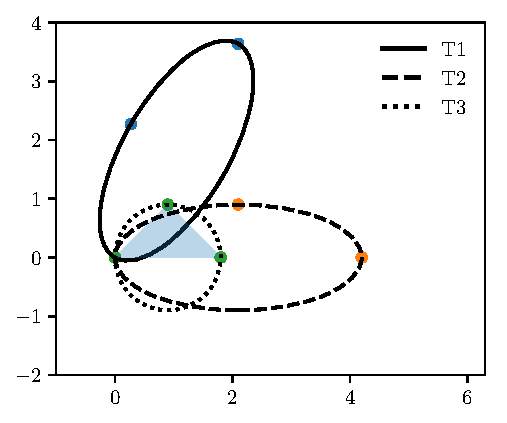
\includegraphics{tex/figures/scripts/circumscribed-circle}
	\fautor
	\label{fig:circumscribed-circle}
\end{figure}
\begin{equation}\label{eq:trpnts}
\varphi(p, \theta)=\left[\begin{array}{cc}
\frac{b}{a}&0\\
0&1
\end{array}\right]
\left[\begin{array}{cc}
\cos{\theta}&\sin{\theta}\\
\sin{\theta}&-\cos{\theta}
\end{array}\right]\left[\begin{array}{c}
p_x\\
p_y
\end{array}\right].
\end{equation}

Then, the problem to be solved is finding a circumscribed circle of the triangle formed by the points $(0, 0), \varphi(v, \theta)$ and $\varphi(w, \theta)$, such that the circle has radius $b$. As, for three non-colinear fixed points, there is always an unique circumscribed circle for the triangle formed by those three points, the only variable to be determined ends up being the angle of rotation $\theta$.

Let $A(\theta)$ be the area of the triangle formed by the points $(0, 0), \varphi(v, \theta)$ and $\varphi(w, \theta)$--note that the transformation does not preserve distance or area. Then, the radius $R$ of the circumscribed circle is given by \autoref{eq:circumscribed_circle} \cite[p.~189]{johnson1960}.

\begin{equation}\label{eq:circumscribed_circle}
R = \dfrac{\norm{\varphi(v, \theta)}\norm{\varphi(w, \theta)}\norm{\varphi(v, \theta)-\varphi(w, \theta)}   }{4A(\theta)}.
\end{equation}

Imposing the radius to be equal $b$ and squaring to eliminate the square roots present in the Euclidean distance, a function $\xi : [0, \pi) \mapsto \mathbb{R}_{>0}$ is defined by \autoref{eq:circumscribed_circle_b}. Note that, the problem now becomes the one of finding every $\theta \in [0, \pi)$, such that $\xi(\theta)=0$.

\begin{equation}\label{eq:circumscribed_circle_b}
\xi(\theta) = 16b^2A(\theta)^2 - \norm{\varphi(v, \theta)}^2\norm{\varphi(w, \theta)}^2\norm{\varphi(v, \theta)-\varphi(w, \theta)}^2.
\end{equation}

According to \citeonline[p.~150]{powell}, any function of the form $\{\cos^j{x}\sin^k{x} : j, k \in \mathbb{N}\}$ can be written as a real trigonometric polynomial of degree $j+k$ which can have up to $2(j+k)$ different roots in the interval $[0, 2\pi)$. The reason to bring up this fact is that $\xi(\theta)$ can be written as $\sum_i^M c_i \cos^{j_i}(\theta)\sin^{k_i}(\theta)$, for some $M \in \mathbb{N}$ and $c_1, \dots, c_m \in \R$, which implies that it can have up to $2$ times its degree, denoted by $\max_{i\in \{1, \dots, M\}}$, zero.

 To show that, just note that it is possible to write $\norm{\varphi(v, \theta)}^2$ and $A(\theta)^2$ in that form, as it can be seen on \autoref{eq:dd} and \autoref{eq:dd2}, combine the parts as $\xi(\theta)$ is just addition and multiplication of terms in that form. It is also possible to see that the term of higher the degree of $\xi(\theta)$ is the multiplication of the three squared distances, as $\norm{\varphi(v, \theta)}^2$ has degree $2$ the degree of $\xi(\theta)$ is $6$.


\begin{align}\label{eq:dd}
	\norm{\varphi(v, \theta)}^2 = (v_x\frac{b}{a}\cos\theta + v_y\frac{b}{a}\sin\theta)^2 + (v_x\cos\theta - v_y\sin\theta)^2\\
	\label{eq:dd2} A(\theta)^2=\dfrac{1}{4}\det\left(
	\begin{array}{cc}
		v_x\frac{b}{a}\cos\theta + v_y\frac{b}{a}\sin\theta&v_x\cos\theta - v_y\sin\theta\\
		w_x\frac{b}{a}\cos\theta + w_y\frac{b}{a}\sin\theta&w_x\cos\theta - w_y\sin\theta
	\end{array}\right)^2
\end{align}

Because ellipses are symmetrical with respect to their major-axis, and any rotation in the interval $[0, \pi)$ is identical to a rotation in $[\pi, 2\pi)$, the number of different solutions is cut in half.
Therefore, the number of angles of rotation and centers that an ellipse of fixed shape can be placed, so it has three fixed points on its border is limited to $6$.

A possible approach to find all the roots of a high-degree polynomial is to find all the eigenvalues of its companion matrix\cite{horn}. There are methods that do that with the observation that roots not close to the origin are susceptible to large errors and some times can not be found. This was experienced in some instances where the method could not find any roots which were priorly known.
Therefore, Because there is no closed formula to find roots of polynomials of degree $12$ \cite{skopenkov2015}, and root-finding iterative methods, such as Newton's method, generally are not convergent for polynomials of degree $4$ or more \cite{mc1}, this approach is only useful to show the limitedness of the set of solutions. In the next section we present a method to approximate the roots of \autoref{eq:circumscribed_circle_b}.

\subsection{A method for E3PNT}

In this section we present a method for E3PNT and we try to make a case of it being correct, however, a proof is left as future work.

The idea of the method is to let two of the three points be fixed on the border of the ellipse and vary the angle to find it when the third point hits the border of the ellipse.

Let $u$ and $v$ be the pair out of the three points that are most distant from each other, also let $\theta_u \in [0, \pi)$ be the greatest $(E, u, v)$-feasible angle. Given an angle $\theta \in [0, \theta_u]$, let $q_\theta\in\R^2$ be a center of $E$, such that $\{u, v\} \subset \tilde{E}(q_\theta, \theta)$. Note that in general, there are two such centers, they could be told apart by their $y$-coordinate, and the method needs to be executed for both of them separately.
Then, a function $\rho : [0, \theta_u] \mapsto \R$ is defined to be the elliptical norm of the point $w$ with respect to $E(q_\theta, \theta)$.

\begin{equation}\label{eq:rho}
\rho(\theta) = \dfrac{\left((w-q_\theta)^T\left(\begin{array}{c}
	\cos{\theta}\\
	\sin{\theta}
	\end{array}\right)\right)^2}{a^2}+
\dfrac{\left((w-q_\theta)^T\left(\begin{array}{c}
	\sin{\theta}\\
	-\cos{\theta}
	\end{array}\right)\right)^2}{b^2}
\end{equation}

The angles such that \autoref{eq:rho} is equal to $1$ are the ones that are part of the solution and achieve three points on the border of the ellipse. From now on, a method is presented that tries to find those points in a efficient way. We conjecture that \autoref{eq:rho} is unimodal by parts, and we present a method that takes advantage of that.

